% -----------------------------------------------------------------------------
% A thesis for the Master of Computer Engineering
% Leonard Berresheim
% 2021/2022
% -----------------------------------------------------------------------------
\documentclass[11pt,a4paper]{book}
\usepackage{mathesis}

% -----------------------------------------------------------------------------
% Packages
% -----------------------------------------------------------------------------
\usepackage{textpos}
\usepackage{xcolor}
\usepackage{graphicx}
\usepackage{amsmath}
\usepackage{hyperref}

\definecolor{htwgreen}{RGB}{118,185,0}
\graphicspath{./images}

% -----------------------------------------------------------------------------
% Front Matter
% -----------------------------------------------------------------------------
\begin{document}


\begin{titlepage}

    \begin{center}
        
\includegraphics[width=0.28\textwidth,keepaspectratio]{images/htw_logo.jpg}
        \vspace{0.3cm}
        \par\noindent\rule{\textwidth}{0.4pt}
        \\
        \vspace{0.7cm}
        \LARGE
        {\color{htwgreen}
        \textbf{Active Noise Control in Spatial Domains}
        }
        \par\noindent\rule{\textwidth}{0.4pt}
        \\
        \Large
        \vspace{0.3cm}
        Masterarbeit
        \\
        \vspace{2cm}
        \small
        Name des Studiengangs
        \vspace{0.4cm}
        \\
        \Large
        Computer Engineering
        \vspace{0.4cm}
        \\
        {\color{htwgreen}
        \textbf{Fachbereich 1}
        }
        \vspace{0.4cm}
        \\
        \small
        vorgelegt von
        \vspace{0.4cm}
        \\
        \Large
        Leonard Berresheim
        \\
        \vspace{4cm}
        \small
        Datum
        \vspace{0.4cm}
        \\
        \normalsize
        Berlin, TT.MM.JJJJ
        \vspace{1.4cm}
        \\
        \Large
        Erstgutachter: Prof. Dr. rer. nat. Andreas Zeiser\\
        \vspace{0.4cm}
        Zweitgutachter: Prof. Dr. rer. nat. Frank Bauernöppel\\
        
        \vfill
    \end{center}
\end{titlepage}
\frontmatter
\input{text/1-originality}
\input{text/2-acknowledgements}
% -----------------------------------------------------------------------------
% Abstract
% -----------------------------------------------------------------------------
\chapter{\centering Abstract}

With the continuing urbanization of modern life, spaces of quiet have become exceedingly rare. Highways have taken over the country side, the cities are overloaded with cars, the sky is pervaded by planes and the oceans have succumbed to cruise ships and freighters. And these vehicles on which we have made our selves dependant are not subtle in their making of commotion.
And therefore, as the only solution our contemporary human society has to offer to solve problems caused by technology is even more technology, active noise control comes into play, allowing us to create secluded spaces of silence in a world of rumble.
\tableofcontents
\listoffigures

% -----------------------------------------------------------------------------
% Main Matter
% -----------------------------------------------------------------------------
\mainmatter
% -----------------------------------------------------------------------------
% Introduction
% -----------------------------------------------------------------------------
\chapter{Introduction}
\label{chap:introduction}


\section{Intention}
    \begin{itemize}
        \item Simulate an active noise control system. 
    \begin{itemize}
        \item Simulate the dispersion of an acoustical source in a 3D space
        \item Simulate a simple ANC-(feedback) system (1 secondary source, 1 error microphone) using existing algorithms
        \item Simulate and advanced ANC system using existing algorithms
    \end{itemize}
        \item Research the possible use of new algorithm i.e. genetic algorithms or Convolutional Neural Networks
\end{itemize}



\large{Feedforward System}\\
For a feedforward system, the time it takes for the primary acoustic or vibration signal to travel from the reference sensor location to the error sensor location, must be greater than the processing time of the controller, plus the time delay associated with control source electro-acoustics, plus the time taken for the signal to travel from the control sources to the error sensors.\cite{Fuller1995}

Unfortunately, the physical acoustic or vibration system to
be controlled rarely remains the same for very long (as even small changes in temperature or
flow speed change the speed of sound, resulting in phase errors between the desired and
actual control signals).\cite{Fuller1995}

Problems can be caused by the reference signal being contaminated by the control source that is transmitted upstream.\cite{Fuller1995}

When designing a feedforward system it is necessary to provide on-line system identification of the electro-acoustic transfer functions of the control sources and error microphones and the acoustic delay between them or else design a complex controller that does not need this information. This latter alternative could require the use of complex filter structures such as neural networks or non-linear adaptive algorithms such as genetic algorithms.\cite{Fuller1995}

The runtime of a genetic algorithms is dependant on the run-time of it's fitness function.\cite{https://www.youtube.com/watch?v=uQj5UNhCPuo}

\large{Feedback System}\\
Feedback systems are used to reduce the transient response of systems, thus returning the system to its unperturbed state as quickly as possible.\cite{Fuller1995}


A feedforward system should be used when it's possible to get a suitable reference signal, as the performance of feedforward systems is, in general, superior to feedback systems \cite{Fuller1995}
% -----------------------------------------------------------------------------
% Fundamentals
% -----------------------------------------------------------------------------
\chapter{Fundamentals}
\label{chap:fundamentals}

\section{Propagation of sound}
An acoustic wave is essentially a change in pressure. A local pressure change causes the surrounding medium to compress which in turn causes pressure changes thus leading to the propagation of an acoustic wave. This compression leads to a displacement of the particles in the medium.\\The linear wave equation can be used to describe such an acoustic wave. In reality the acoustic wave equation is non linear but for this application the linear approximation to the wave equation is a good model.\cite{Acoustic}\\
\subsection{Linearity}
Viewing acoustics as a linear phenomenon is very appealing due to the principle of superposition roughly depicted by following relation
\begin{equation}
    \mathcal{L}(af_1+bf_2) = a\mathcal{L}(f_1) + b\mathcal{L}(f_2),
\end{equation}
where
$f_1$ and $f_2$ are two causes,\\
$\mathcal{L}(f)$ is the set of possible computational steps that predict the effect of $f$.\\
Thus a complex sound field stemming from multiple sources can be regarded as the sum of sound fields produced by each source individually. In the same way a complex wave can be analyzed by each frequency separately. Nevertheless this acoustic model only represents an approximation.\cite{}
\\
The following three laws are used to develop the wave equation.
\subsection{Equation of State}
The equation of state relates changes in pressure and density. It is determined by thermodynamic properties and dependant upon the material (e.g. air):
\begin{equation}
    p = \mathbf{B}s = \rho_0c^2s,
\end{equation}
where 
$\mathbf{B}=\rho_0(\frac{\partial P}{\partial \rho})_{\rho_0}$ is the adiabatic bulk modulus,\\
$\rho$ in $kg/m³$ is the density,
$\rho_0$ is the undisturbed density,\\
$p$ in $Pascal$ where $1Pa = 1 N/m^2 = 1kg/s^2/m$ is the pressure,\\
$P$ is the instantaneous pressure,\\
$c$ in $m/s$ is the speed of sound,\\
$s = \frac{\rho-\rho_0}{\rho_0}$ is the condensation 
\subsection{Equation of Continuity}
The equation of continuity depicts the conservation of mass:
\begin{equation}
    \frac{\partial\rho}{\partial t} = -\rho_0\nabla\cdot\Vec{u},
\end{equation}
where\\
$t$ is time,\\
$\nabla$ is the Laplace operator.\\
$\Vec{u} = \frac{\partial\Vec{\xi}}{\partial t}$ is the particle velocity,\\
$\Vec{\xi}$ is the particle displacement,\\
$\Vec{x}$ is the particle position.
\subsection{Equation of Motion}
The Equation of motion describes how a pressure variation generates a force that causes particle motion:
\begin{equation}
    -\nabla p = \rho_0 \cdot \frac{\partial\Vec{u}}{\partial t}
\end{equation}
\subsection{Wave Equation}
The wave equation or the equation of propagation of acoustic pressure can be derived from the three preceding equations:
\begin{equation}
    \frac{1}{c^2}\frac{\partial^2p}{\partial t^2} = \nabla^2p
\end{equation}
in Cartesian coordinates $(x,y,z)$:
\begin{equation}
    \frac{1}{c^2}\frac{\partial^2p}{\partial t^2} = \frac{\partial^2p}{\partial x^2} + \frac{\partial^2p}{\partial y^2} + \frac{\partial^2p}{\partial z^2},
\end{equation}
in Polar coordinates $(r,\theta, z)$:
\begin{equation}
    \frac{1}{c^2}\frac{\partial^2p}{\partial t^2} = \frac{\partial^2p}{r^2\partial \theta^2} + \frac{\partial^2p}{\partial r^2} + \frac{1}{r}\frac{\partial^2p}{\partial r} + \frac{\partial^2p}{\partial z^2},
\end{equation}

\subsection{Spherical Wave Equation}

For now we assume the acoustic source to be a point source, it can thus be represented as a spherical wave. Furthermore we assume "spherical symmetry" i.e. the pressure and particle velocity equal for the same $r$, the distance from the 'origin' of the spherical wave. The wave equation for the spherically symmetric wave is\cite{Waves2004}:
\begin{equation}
    \frac{\partial^2rp(r,t)}{\partial r^2} = \frac{1}{c^2}\frac{\partial^2rp(r,t)}{\partial t^2}.
\end{equation}
\subsubsection{General Solution to the Spherical Wave Equation}
A general solution to the Wave equation is given by the pressure wave emitted by a single frequency point source of acceleration in free space\cite{Allen1979}:
\begin{equation}
    p(\omega,\Vec{x},\Vec{x}') = \frac{e^{i\omega(\frac{r}{c}-t)}}{4\pi r}\quad\quad for\quad r > 0,
\end{equation}
where\\
$p$ is the pressure,\\
$\omega=2\pi f$,\\
$f$ is the frequency,\\
$r=|\Vec{x}-\Vec{x}'|$ is the distance from source to receiver,\\
$\Vec{x}$ is the source location $(x,y,z)$,\\
$\Vec{x}'$ is the receiver location $(x',y',z')$,\\
$i=\sqrt{-1}$.\\


    

\section{Spherical Harmonics}
"The spherical harmonics are a set of orthogonal spatial basis functions that can be utilized
to decompose any arbitrary function defined on the sphere."\cite{Samarasinghe2018}\\
A homogeneous incident wave field $v(\mathbf{x},k)$ observed at $\mathbf{x}$ can thus be decomposed into\cite{Zhang2019}:
\begin{equation}
    v(\mathbf{x},k)=\sum_{u=0}^\infty \sum_{m=-u}^u\beta_{um}(k)j_u(kr)\Upsilon_{um}(\Phi_x,\Psi_x),
\end{equation}
for any location with spherical coordinates $\mathbf{x}=(x,\Phi_x,\Psi_x)$\\
where\\
$k=2\pi f/c=$ the wave number,\\
$f=$ the frequency,\\
$c=$ the speed of sound,\\
$j_u(.)=$the spherical Bessel function of order $u$,\\
$\beta_um(k)=$ the wave field in the wave domain.\\ 
$\Upsilon_{um}(.)=$ the spherical harmonics,\\
The spherical harmonics function of order $n$ and mode $m$ is defined by\cite{Samarasinghe2018}
\begin{equation}
    \Upsilon_{um}(\Phi_x,\Psi_x) = \mathbf{P}_{n|m|}(cos(\Phi_x))\frac{1}{\sqrt{2\pi}}e^{im\Psi_x},
\end{equation}
where\\
$\mathbf{P}_{n|m|}(cos(\Phi_x))=$ the associated Legendre polynomials.
\section{Simulating an acoustic source in 3D - space}
Other Methods for simulating rooms acoustics among others:
\begin{itemize}
    \item ray/beam tracing
    \item boundary and finite element methods
    \item digital waveguide meshes
    \item spatial sound decomposition based methods
The image source method still remains a sought-after technique.\cite{Samarasinghe2018}
\end{itemize}

\subsection{Image Source Method}
The image model is a method that allows the computation of a source-to-receiver acoustic transfer function in an enclosed 3D-space. Within this method an acoustic wave produced by a source, when crossing a wall, produces an image which then itself is considered as a source for further computation. In a room with several walls each image then also produces an image.\cite{Allen1979}
\\\\
The exact solution to the wave equation in a rectangular, rigid-wall, room is given by the rooms impulse response function also known as the time domain Green's function\cite{Allen1979}:
\begin{equation}
    p(t,\mathbf{X},\mathbf{X'})=\sum_{p=1}^8\sum_{r=-\infty}^\infty\frac{\delta[t-\frac{|\mathbf{R_p}+\mathbf{R_r}|}{c}]}{4\pi|\mathbf{R_p}+\mathbf{R_r}|},
\end{equation}
where\\ 
$c=$ the speed of sound,\\
$\mathbf{R_p}$ represents the eight vectors given by the eight permutations over $\pm$ of
\begin{equation}
    \mathbf{R_p}=(x\pm x', y\pm y', z\pm z')
\end{equation}
r is the integer vector triplet $(n,l,m)$, and
\begin{equation}
    \mathbf{R_r}=2(nL_x, lL_y, mL_z),
\end{equation}
where $(L_x, L_y, L_z)$ are the room dimensions.
\\
\\
In case of non-rigid walls, the solution to the wave equation becomes more complicated and is only conceivable under the assumption that the wall impedance is proportional to $sec(\theta)$, where $\theta$ is the angle incidence of a plane wave with respect to the wall normal, resulting in the Sabine energy absorption coefficient $\alpha$ for a uniform reflection coefficient $\beta$ on a given wall of the form\cite{Allen1979}:
\begin{equation}
    \alpha=1-\beta^2.
\end{equation}
The modified room impulse response transforms into:
\begin{equation}
    p(t,\mathbf{X},\mathbf{X'})=\sum_{p=1}^8\sum_{r=-\infty}^\infty
    \beta_{x1}^{|n-q|}\beta_{x2}^{|n|}\beta_{y1}^{|i-j|}\beta_{y2}^{|i|}\beta_{z1}^{|m-k|}\beta_{z2}^{|m|}
    \frac{\delta[t-\frac{|\mathbf{R_p}+\mathbf{R_r}|}{c}]}{4\pi|\mathbf{R_p}+\mathbf{R_r}|},
\end{equation}
where\\
$p=(q,j,k)$ and $r=(n,l,m)$ are integer 3-vector,\\
$\mathbf{R_p}$ is now expressed in terms of $p$ as
\begin{equation}
    \mathbf{R_p}=(x-x'+2qx', y-y'+2jy,z-z'+2kz').
\end{equation}


\subsection{Spherical Harmonics Based Image Source Method}
The image source method was developed under the assumption that both source and receiver are omnidirectional. As loudspeaker are inherently directional and the use of directional microphones is increasing it is expedient to use a different approach. By modeling the transducers in the spherical harmonics domain with a more realistic directivity pattern it is possible to achieve a more accurate simulation of room acoustics.\cite{Samarasinghe2018}\\
The spherical harmonics based image source method also known as the generalised image source method is given by
\begin{equation}
    \mathbf{P}(k,\mathbf{x}_s,\mathbf{z}^{(r)} = \sum_{v=0}^V\sum_{u=-v}^v\sum_{n=0}^N\sum_{m=-n}^n\sum_{\mathbf{p}=0}^1\sum_{\mathbf{r}=-\infty}^\infty\beta_{nm}(k)\\
    \times (-1)^...
\end{equation}
\\
\\The advantages of the image source method are its relatively simple algorithmic implementation, its high degree of flexibility - many parameter can be set within the software - as well as its ability to generate a good approximation of the room impulse response. It nevertheless comes with its impediments such as its restriction to rectangular rooms and it's inability to model diffraction.\cite{Samarasinghe2018}
% -----------------------------------------------------------------------------
% Solution Approach
% -----------------------------------------------------------------------------
\chapter{Solution Approach}
\label{chap:approach}
The process of \textit{spacial ANC} seeks to reduce the residual signal at any point $\mathbf{x} \equiv \{r,\theta_x, \phi_x\}$ within the region of interest. The residual signal is given by
\begin{equation}
    e(\mathbf{x},k) = v(\mathbf{x},k) + s(\mathbf{x},k),
    \label{eq:residual}
\end{equation}
where\\
$k$ is the wave number,\\
$v(\mathbf{x},k)$ is the primary noise field observed at a point $\mathbf{x}$ i.e. the noise field generated by the noise source and its reverberation in the room.\\
$s(\mathbf{x},k)$ is the secondary noise field i.e. the \textit{anti-}noise field emitted by the set of loudspeakers on behalf of the ANC process.
\section{Primary Noise Field}\label{sec:primary}
The primary noise field can be expressed using the spherical harmonics decomposition in (\ref{eq:wave_field_decomposition}). Within the region of interest the noise field can be approximated with a finite number of modes with truncation order of $N = \lceil ekR_1/2\rceil$ \cite{Kennedy2007}. The primary noise will therefore be expressed by
\begin{equation}
    v(\mathbf{x},k) \approx \sum_{u=0}^N \sum_{m=-u}^u\beta_{um}(k)j_u(kr)Y_{um}(\theta_x,\phi_x),
    \label{eq:primary_noise_field}
\end{equation}
where\\
$R_1$ is the radius of the quiet zone,\\
$\beta_{um}$ are the harmonic coefficients representing the primary noise field in the wave domain.\\\\
Putting the harmonic coefficients in vector form we get:
\begin{equation}
    \boldsymbol{\beta}(k) = [\beta_{0,0}(k),\beta_{1,-1}(k),...\beta_{N,N}(k)]^T
    \label{eq:primary_coefs_vector}
\end{equation}

\section{Secondary Noise Field}
Applying a simple loudspeaker model the secondary noise field can be represented by \cite{Zhang2019}
\begin{equation}
    s(\mathbf{x},k) = \sum_{l=1}^Ld_l(k)G(x|\mathbf{y}_l,k),
    \label{eq:secondary_noise_field_atf}
\end{equation}
where\\
$d_l(k)$ is the driving signal for the $l^{th}$ loudspeaker,\\
$\mathbf{y}_l$ is the location of the $l^{th}$ loudspeaker,\\
$G(x|\mathbf{y}_l,k)$ is the acoustic transfer function between the $l^{th}$ loudspeaker and the observation point $\mathbf{x}$.\\\\
\textit{Nota}\\
The acoustic transfer function $G(x|\mathbf{y}_l,k)$ includes the reflections stemming from the walls of the room.\\\\
Similar to the primary noise field in (\ref{eq:primary_noise_field}) the secondary noise field can be approximated by
\begin{equation}
    s(\mathbf{x},k) \approx \sum_{u=0}^N \sum_{m=-u}^u\gamma_{um}(k)j_u(kr)Y_{um}(\theta_x,\phi_x),
    \label{eq:secondary_noise_field}
\end{equation}
where\\
$\gamma_{um}$ are the harmonic coefficients representing the secondary noise field in the wave domain.\\\\

The acoustic transfer function in (\ref{eq:secondary_noise_field_atf}) can be expressed in the wave domain as \cite{Betlehem2005}
\begin{equation}
    G(x|\mathbf{y}_l,k) \approx \sum_{u=0}^N \sum_{m=-u}^u\eta^{(l)}_{um}(k)j_u(kr)Y_{um}(\theta_x,\phi_x)
    \label{eq:ATF_wavedomain}
\end{equation}
where\\
$\eta^{(l)}_{um}$ are the harmonic coefficients representing the acoustic transfer function for the $l^{th}$ loudspeaker in the wave domain.\\\\
By substituting (\ref{eq:secondary_noise_field}) and (\ref{eq:ATF_wavedomain}) into (\ref{eq:secondary_noise_field_atf}) the harmonic coefficients secondary source can also be represented by
\begin{equation}
    \gamma_{um}(k) = \sum_{l=1}^Ld_l(k)\eta_{um}^{(l)}(k).
\end{equation}
in matrix form:
\begin{equation}
    {\boldsymbol{\gamma}}(k)=\boldsymbol{\eta}(k) \mathbf{d}(k),
\end{equation}
where\\
\begin{equation}
    \boldsymbol{\eta}(k) = 
    \begin{bmatrix}
        \eta_{00}^{(1)}(k) & \eta_{00}^{(2)}(k) & \hdots & \eta_{00}^{(L)}(k)\\
        \eta_{-11}^{(1)}(k) & \eta_{-11}^{(2)}(k) & \hdots & \eta_{-11}^{(L)}(k)\\
        \vdots & \vdots & \ddots & \vdots\\
        \eta_{NN}^{(1)}(k) & \eta_{NN}^{(2)}(k) & \hdots & \eta_{NN}^{(L)}(k)
    \end{bmatrix}
    \label{eq:secondary_coef_vector}
\end{equation}
and\\
\begin{equation}
    \boldsymbol{d}(k) = [d_1(k),...,d_L(k)]^T.
\end{equation}
The acoustic transfer function for each loudspeaker to each microphone can be computed knowing the position of the loudspeakers and dimensions of the room, the exact working of this is discussed in \textit{section \ref{sec:Simulation}}. Subsequently the method explained in \textit{section \ref{sec:sampling}} can be used to determine the harmonic coefficients $\eta^{(l)}_{um}(k)$ for the acoustic transfer function. The same can be done to determine the harmonic coefficients $\beta_{um}$ for the primary noise field.\\\\
What remains to be done is setting the driving signal $d_l(k)$ for each loudspeaker appropriately to emit a secondary noise field $s(\mathbf{x},k)$ inciting a reduction of the residual noise e(\mathbf{x},k) in the region of interest thus resulting in a quiet zone.


\section{Matching Noise Fields}\label{sec:matching}
Having determined the primary noise field and the acoustic transfer function in the wave domain one method of deriving the driving signal for the loudspeakers is simply to match the secondary noise field harmonic coefficients to the primary noise field harmonic coefficients\cite{Zhang2019}:
\begin{equation}
    \boldsymbol{\eta}(k)\mathbf{d}(k)=-\boldsymbol{\beta}(k).
    \label{eq:matching}
\end{equation}
When choosing the number of loudspeakers there's three possible cases that determine the solution to the harmonic coefficients matching:

\subsubsection{Case 1: $L = (N + 1)^2$}
When the number of loudspeakers $L$ is equal to the number of modes $(N+1)^2$ then there's one unique solution to \ref{eq:matching} given by\cite{Zhang2019}:
\begin{equation}
    \mathbf{d}(k) = -(\boldsymbol{\eta}(k))^{-1}\boldsymbol{\beta}(k),
\end{equation}
where\\
$(.)^{-1}$ is the inverse matrix.\\\\
\textit{Memoriae}\\
The number of modes is dependant on the frequency and the radius of the region of interest.
\subsubsection{Case 2: $L > (N + 1)^2$}
When the number of loudspeaker is greater than the number of modes then there's either no solution or an infinite number of solutions\cite{Zhang2019}.
\subsubsection{Case 3: $L < (N + 1)^2$}
This case is worthy of further consideration as it is the most viable for implementing a realistic \textit{spatial ANC} system. When the number of loudspeakers is lesser then the number of modes then there's is an exact solution only in a very special case\cite{Zhang2019}. In general however \textit{(and this will be of greater interest)} there's no exact solution and an approximation is necessary.
\subsection{Least Squares Method}

\subsubsection{Wave-Domain Least Square Method}
Applying the least square method on (\ref{eq:matching}) for \textit{case 3} comes back to solving the problem
\begin{equation}
    min||\boldsymbol{\eta}(k)\boldsymbol{d}(k)-(-\boldsymbol{\beta}(k))||^2
\end{equation}
The optimal solution to this problem is\cite{Zhang2019}
\begin{equation}
    \boldsymbol{d}(k) = -(\boldsymbol{\eta}(k))^\dagger\boldsymbol{\beta}(k),
\end{equation}
where\\
$(.)^\dagger$ is the pseudoinverse matrix.
% -----------------------------------------------------------------------------
% Implementation
% -----------------------------------------------------------------------------
\chapter{Implementation}

As noted before the ANC system has solely been implemented in the simulation environment Matlab. The system consist of several subsystems. These subsystems will be elaborated step by step and their functioning will be demonstrated.\\
The complete source code can be found in the \color{blue}\href{https://github.com/leonardberresheim/MA---Active-Noise-Control-in-Spatial-Domains/tree/main/Matlab}{projects github repository} \color{black} and is free to use, change and share without restrictions.



\section{Spherical Harmonics Decomposition}
The accuracy of the spherical harmonics decomposition in (\ref{eq:primary_noise_field}) with it's truncation degree will be demonstrated using a plane wave \textit{(see figure \ref{fig:planeWaveExp}}) as the exact harmonic coefficients can be calculated using (\ref{eq:plane_wave_coefficients}).
\begin{figure}
    \centerline{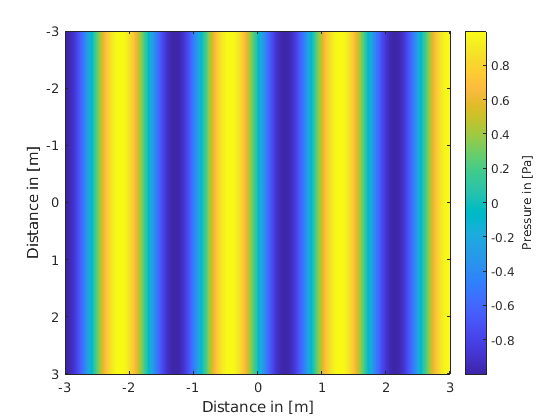
\includegraphics{LaTeX/images/plots/plane_Wave_exponent_form.png}}
    \caption{Plane wave in exponent form}
    \label{fig:planeWaveExp}
\end{figure}

\begin{figure}
    \centerline{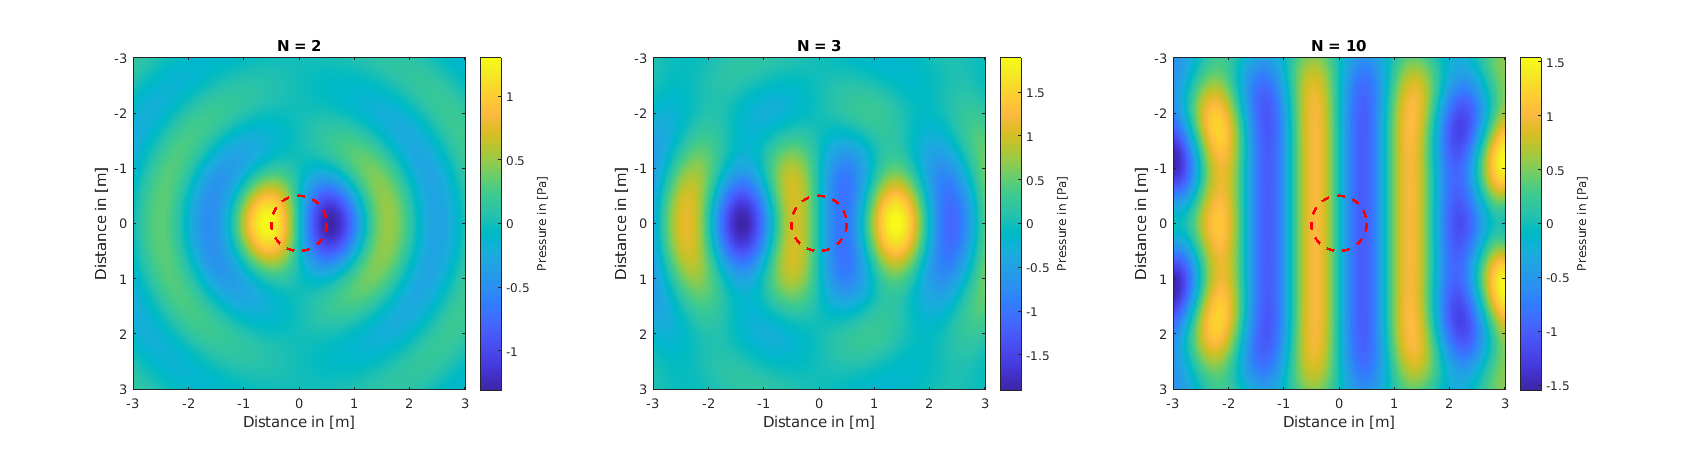
\includegraphics[width=\paperwidth]{LaTeX/images/plots/Plane_wave_harmonics_form.png}}
    \caption{Plane wave in harmonics form for number of modes 2, 3 and 10}
    \label{fig:planeWaveHarmonics}
\end{figure}
When increasing the number of modes the resulting noise field gets closer and closer to the original plane wave in figure \ref{fig:planeWaveExp} as can be seen in figure \ref{fig:planeWaveHarmonics}. However only the quiet zone (\textit{marked as a red circle}) is of interest and with a higher number of modes the number of required loudspeakers increase as well as the computation time. In fact figure \ref{fig:planeWaveHarmonicsError} shows that in the region of interest the accuracy of the spherical harmonics decomposition for $N = 3$ is already adequate.
\begin{figure}
    \centerline{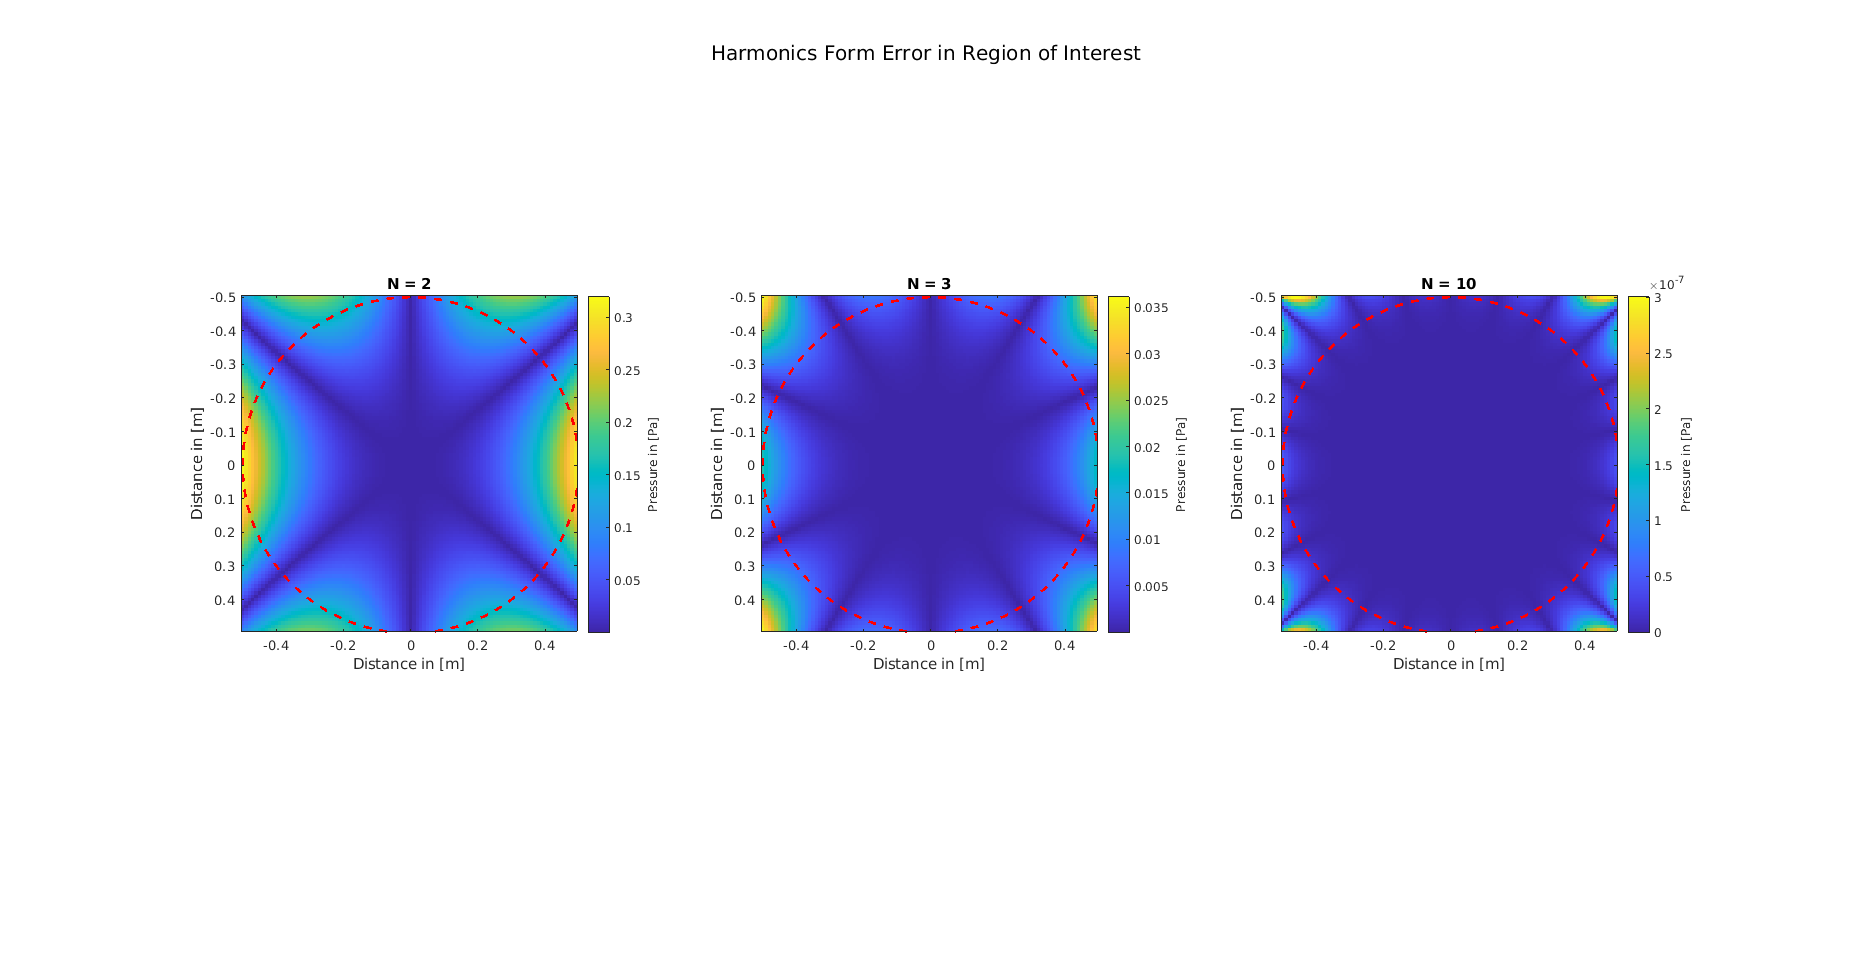
\includegraphics[width=\paperwidth]{LaTeX/images/plots/Plane_wave_harmonics_form_Error.png}}
    \caption{Error of the plane wave in harmonics form within region of interest for number of modes 2, 3 and 10}
    \label{fig:planeWaveHarmonicsError}
\end{figure}
\\
\\
\textit{Nota}\\
Only the imaginary part is plotted here as the behavior of the real part of the wave is analogous.
\section{Spherical Microphone Array}
The spherical microphone array is setup around the region of interest according to the Gaussian sampling scheme discussed in \textit{section \ref{sec:Gaussian}} with $2(N+1) = 8$ microphones on the azimuth angle in line with (\ref{eq:azimuth_sample}) and $(N + 1) = 4$ microphones on the elevation angle in line with (\ref{eq:elevation_sample}) resulting in a total of $2(N + 1)^2 = 32$ microphones arranged on the sphere \textit{(see figure \ref{fig:MicrophoneArray}})
\begin{figure}
    \centerline{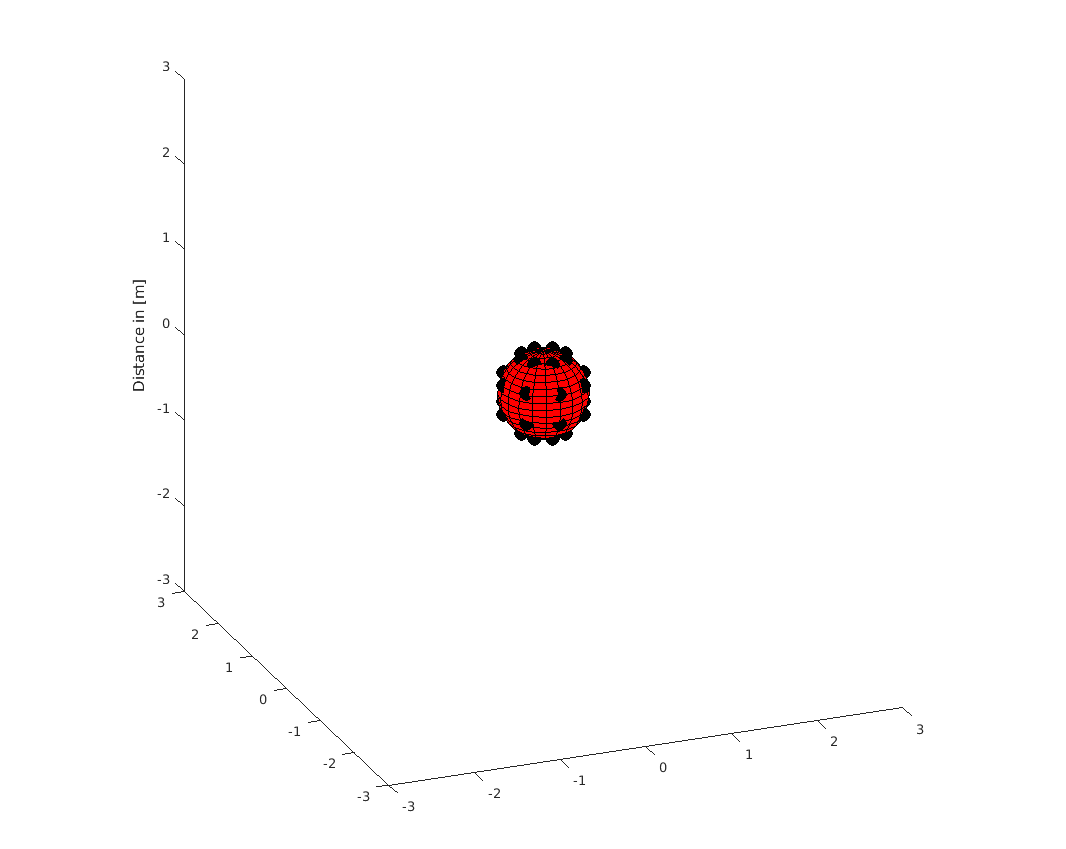
\includegraphics[width=\paperwidth]{LaTeX/images/plots/MicrophoneArray.png}}
    \caption{Spherical microphone array arranged according to the Gaussian sampling scheme}
    \label{fig:MicrophoneArray}
\end{figure}
\section{Approximation of Harmonic Coefficient}
Applying the Gaussian sampling scheme discussed in \textit{section \ref{sec:Gauss}}, the sampling weights are set according to (\ref{eq:gauss_weights}) and the harmonic coefficients for the noise field generated by the plane wave are approximated using (\ref{eq:gauss_harmonic_coefficients}).


\begin{figure}
    \centerline{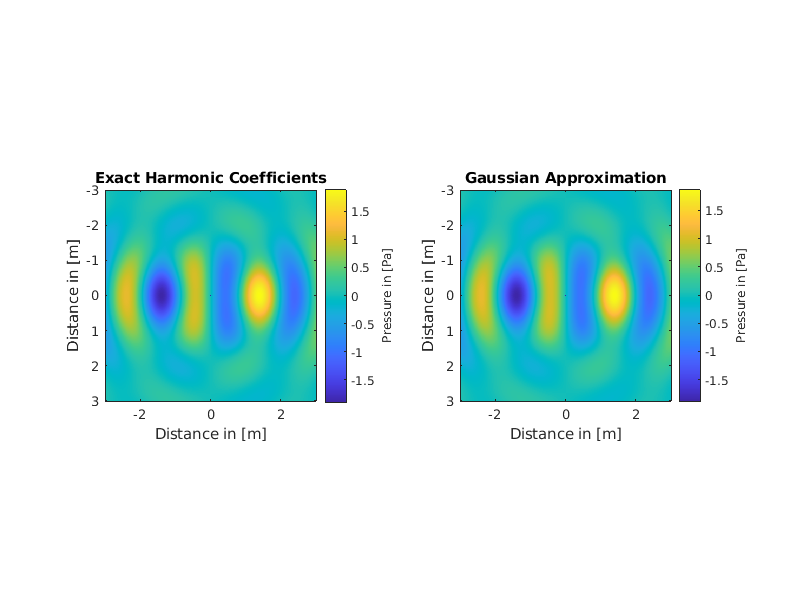
\includegraphics[width=\paperwidth]{LaTeX/images/plots/Gauss_Approcimation.png}}
    \caption{Plane wave noise field approximation in the wave domain with exact harmonic coefficients and Gaussian sampling approximation for N = 3}
    \label{fig:GaussianApproximation}
\end{figure}

The resulting noise field approximation using the Gaussian sampling scheme appears very similar to the exact noise field approximation\textit{(see figure \ref{fig:GaussianApproximation}}.\\
Surprisingly the error of the Gaussian approximation in regards to the actual plane wave is lesser at the corners than for the exact approximation as can be seen in figure \ref{fig:GaussianApproximationError}.\\\\

\textit{Nota}\\
By \textit{exact} the analytical solution to the harmonic coefficient from (\ref{eq:plane_wave_coefficients}) in consideration of the truncation order of $N = 3$ is meant. 


\begin{figure}
    \centerline{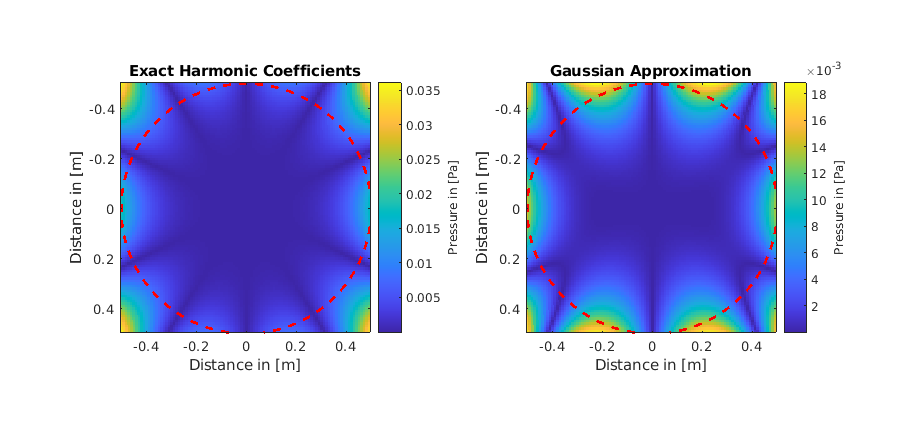
\includegraphics[width=\paperwidth]{LaTeX/images/plots/Gauss_Approximation_Error.png}}
    \caption{Error for the plane wave noise field approximation in the wave domain with exact harmonic coefficients and Gaussian sampling approximation for N = 3}
    \label{fig:GaussianApproximationError}
\end{figure}

\section{Simulation Setup}
The simulation setup is set in accordance with \cite{Zhang2019}. The environment is modeled by a \textit{shoebox} room of $6m \times 6m \times 6m$ with reflection coefficients at [0.75,0.8,0.77,0.85,0.1,0.1] which are usual for a common room with relatively high reflection coefficients for the walls and relatively low reflection coefficients for floor and ceiling. The source is modeled as a point source as defined by (\ref{eq:point_source}. For now we assume the noise field to contain only a single frequency component and the point source to emit at a constant magnitude of 10.\\ The region of interest is spherical area of radius $R_1 = 0.5m$ located at the origin which as seen in \textit{section \ref{sec:primary}} leads to a number of modes of $N = \lceil ekR_1/2\rceil = 3$. As depicted in \textit{section \ref{sec:matching}} $(N+1)^2 = 16$ loudspeaker would be necessary to bear an exact solution. But as aforementioned and discussed \textit{Case 3} will be realized in which the number of loudspeaker is lesser and thus an approximation is required. The number of loudspeaker is set to 12 as seen in figure \ref{fig:setup}.

\begin{figure}
    \centerline{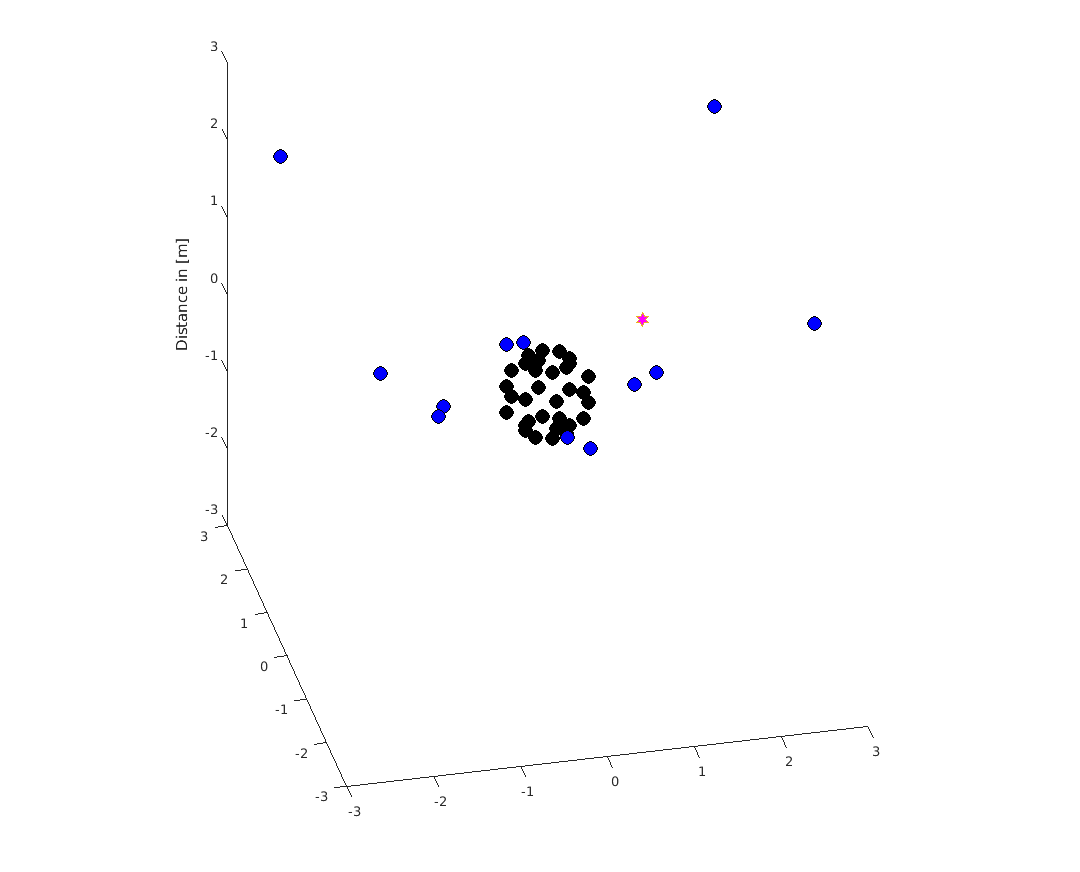
\includegraphics[width=\paperwidth]{LaTeX/images/plots/ANCSetup.png}}
    \caption{Simulation setup, where the blue points are the loudspeaker positions, the pink star is the noise source position and the black points represent the microphones positions}
    \label{fig:setup}
\end{figure}

\section{Point Source Reverberation}



% -----------------------------------------------------------------------------
% Appendices
% -----------------------------------------------------------------------------
\appendix

% -----------------------------------------------------------------------------
% Bibliography
% -----------------------------------------------------------------------------
\backmatter
\bibliographystyle{ieee}
\bibliography{bibliography/Basics}
\end{document}
